\chapter{Zastosowania geometryczne i fizyczne całek}
\label{ma2:ch:integral-applications}

W rozdziałach \ref{ma2:ch:multiple-integrals}
i \ref{ma2:ch:line-integrals} opracowaliśmy
metody obliczania całek wielokrotnych i krzywoliniowych.
Teraz wykorzystamy je do obliczania objętości,
mas, środków masy, momentów bezwładności i pracy.
Jednowymiarowe wzory dla pól, brył obrotowych
i płyt jednorodnych wyprowadzono w
\atlasref{AM1-33::ma1:ch:integral-applications}{AM I, rozdział 33}.
Pracujemy wyłącznie w przestrzeniach euklidesowych.
Wielkości dotyczące powierzchni zostaną rozwinięte
w następnym rozdziale.

\section{Objętość z przekrojów}

\begin{stwierdzenie}[Zasada Cavalieriego]
\label{ma2:prop:applications-cavalieri}
Niech $E\subseteq\R^{m+n}$ będzie mierzalny
względem miary Lebesgue'a. Dla prawie każdego
$x\in\R^m$ przekrój $E_x$ jest mierzalny
względem $\lambda_n$, a funkcja
$x\mapsto\lambda_n(E_x)$, określona jako zero
na wyjątkowym zbiorze miary zero, jest mierzalna.
Wówczas
\[
 \lambda_{m+n}(E)=
 \int_{\R^m}\lambda_n(E_x)\,\mathrm d\lambda_m(x),
 \qquad
 E_x=\{y:(x,y)\in E\}.
\]
Jeżeli dwa zbiory mierzalne mają przekroje
o jednakowych miarach dla prawie wszystkich $x$,
to ich miary są równe.
\end{stwierdzenie}
\begin{proof}
Jest to zastosowanie
\ref{ma2:cor:multiple-sections} do funkcji
charakterystycznych obu zbiorów.
Na wyjątkowych zbiorach miary zero przyjmujemy
wartość zero funkcji miary przekroju.
\end{proof}

\begin{przyklad}[Objętość ostrosłupa i stożka]
\label{ma2:ex:applications-cone}
Niech $D\subseteq\R^2$ będzie zwartą podstawą
o polu $A$, $H>0$, a $p\in\R^2$ rzutem
wierzchołka na płaszczyznę podstawy.
Rozważamy sumę odcinków łączących
punkty $(u,0)$, $u\in D$, z $(p,H)$.
Zbiór $E$ jest zwarty jako obraz
$D\times[0,1]$ przez odwzorowanie ciągłe.
Przekrój na wysokości $z\in[0,H]$ to
\[
 E^z=(1-z/H)D+(z/H)p .
\]
Dla $0\le z<H$ jego pole wynosi
$(1-z/H)^2 A$ na mocy afinicznego wzoru
\ref{ma2:ex:multiple-affine}, a przekrój
wierzchołkowy ma pole zero. Z zasady
\ref{ma2:prop:applications-cavalieri}
\[
 \lambda_3(E)=A\int_0^H(1-z/H)^2\,
 \mathrm d\lambda_1(z)=\frac{AH}{3}.
\]
W szczególności dla kołowej podstawy
promienia $R$ otrzymujemy $\pi R^2H/3$.
Wynik nie zależy od położenia $p$.
\end{przyklad}

\begin{przyklad}[Objętość wspólnej części dwóch walców]
\label{ma2:ex:applications-steinmetz}
Niech $R>0$ i
\[
 E=\{(x,y,z):x^2+z^2\le R^2,\ 
                       y^2+z^2\le R^2\}.
\]
Jest to przecięcie dwóch prostopadłych
walców kołowych. Przy ustalonym $z$,
$|z|\le R$, przekrój jest kwadratem
o boku $2\sqrt{R^2-z^2}$. Zatem
\[
 \lambda_3(E)=\int_{-R}^R4(R^2-z^2)\,
 \mathrm d\lambda_1(z)=\frac{16R^3}{3}.
\]
Nie trzeba tu parametryzować całej
powierzchni ograniczającej bryłę.
\end{przyklad}

\section{Masa, środek masy i symetrie}

\begin{definicja}
\label{ma2:def:applications-mass}
Niech $E\subseteq\R^n$ będzie mierzalny,
a $\rho:E\to[0,+\infty]$ mierzalną funkcją
gęstości. Masa zbioru wynosi
\[
 M=\int_E\rho(x)\,\mathrm d\lambda_n(x).
\]
Zakładając $0<M<\infty$ oraz
$\int_E\|x\|_2\rho(x)\,\mathrm d\lambda_n(x)<\infty$,
określamy środek masy $c\in\R^n$ przez
\[
 c_i=\frac1M\int_E x_i\rho(x)\,
 \mathrm d\lambda_n(x),\qquad i=1,\ldots,n.
\]
Całki współrzędnych istnieją, ponieważ
$|x_i|\le\|x\|_2$. Dla stałej dodatniej
gęstości środek masy nazywamy środkiem
geometrycznym (centroidem).
\end{definicja}

Dla ograniczonego $E$ o skończonej dodatniej
masie warunek skończoności pierwszego momentu
jest automatyczny. Przy nieograniczonym $E$
nie wystarcza sama skończoność masy.

\begin{przyklad}[Skończona masa bez środka masy]
\label{ma2:ex:applications-infinite-first}
Na $E=[1,+\infty)$ połóżmy $\rho(x)=x^{-2}$.
Masa wynosi $1$, ale moment pierwszego rzędu
\[
 \int_1^\infty x\rho(x)\,\mathrm d\lambda_1(x)
 =\int_1^\infty\frac1x\,\mathrm d\lambda_1(x)=+\infty .
\]
Rozbieżność wynika z funkcji pierwotnej $\log x$.
Środek masy nie jest skończoną liczbą.
\end{przyklad}

\begin{twierdzenie}[Środek masy i odwzorowania afiniczne]
\label{ma2:thm:applications-center-affine}
Niech $E,\rho$ spełniają założenia definicji
\ref{ma2:def:applications-mass}. Niech
$T(x)=Ax+b$, gdzie $A$ jest odwracalną
macierzą $n\times n$. Na $T(E)$ połóżmy
$\widetilde\rho=\rho\circ T^{-1}$.
Wówczas
\[
 \widetilde M=|\det A|M,\qquad
 \widetilde c=Ac+b.
\]
Jeśli $T(E)=E$ oraz
$\rho(T(x))=\rho(x)$ prawie wszędzie na $E$,
to $T(c)=c$.
\end{twierdzenie}
\begin{proof}
Stosujemy \ref{ma2:thm:multiple-change}
najpierw do nieujemnych funkcji
$\widetilde\rho$ i $|y_i|\widetilde\rho(y)$.
Otrzymujemy $\widetilde M=|\det A|M$
oraz skończoność pierwszych momentów
bezwzględnych, ponieważ
$\|Ax+b\|_2\le\|A\|\|x\|_2+\|b\|_2$
i założyliśmy skończoność masy i pierwszego
momentu rozkładu początkowego.
Możemy więc zastosować wzór na zamianę
zmiennych również do funkcji ze znakiem
$y_i\widetilde\rho(y)$.
Dla każdej współrzędnej mamy
\[
 \int_{T(E)}y_i\widetilde\rho(y)\,
 \mathrm d\lambda_n(y)
 =|\det A|\int_E (Ax+b)_i\rho(x)\,
 \mathrm d\lambda_n(x).
\]
Dzielimy przez $\widetilde M$ i korzystamy
z liniowości całki skalarnej.
W przypadku symetrii masa i momenty
przekształconego rozkładu są takie same
jak początkowego, więc $T(c)=c$.
\end{proof}
W szczególności dla symetrii względem
płaszczyzny współrzędna prostopadła do niej
jest współrzędną tej płaszczyzny; dla
symetrii środkowej środek masy pokrywa się
ze środkiem symetrii.

\begin{przyklad}[Środek masy półkuli]
\label{ma2:ex:applications-hemisphere}
Rozważmy jednorodną półkulę
$E=\{(x,y,z):x^2+y^2+z^2\le R^2,\ z\ge0\}$
o gęstości $1$.
Z symetrii względem płaszczyzn $x=0$ i $y=0$
mamy $c_x=c_y=0$. Przekrój na wysokości
$z\in[0,R]$ jest kołem pola $\pi(R^2-z^2)$.
Z \ref{ma2:cor:multiple-sections}
\[
 \begin{aligned}
 M&=\pi\int_0^R(R^2-z^2)\,\mathrm d\lambda_1(z)
   =\frac{2\pi R^3}{3},\\
 \int_E z\,\mathrm d\lambda_3(x,y,z)
 &=\pi\int_0^R z(R^2-z^2)\,\mathrm d\lambda_1(z)
   =\frac{\pi R^4}{4}.
 \end{aligned}
\]
Zatem $c=(0,0,3R/8)$.
Dotyczy to pełnej półkuli, a nie samej
powierzchni sferycznej.
\end{przyklad}

\begin{figure}[htbp]
\centering
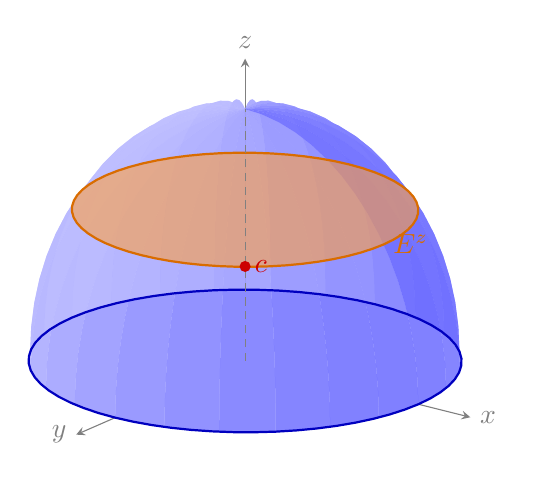
\begin{tikzpicture}[x={(2.2cm,-.55cm)},y={(-1.65cm,-.72cm)},
 z={(0cm,3.2cm)},>=stealth]
 \draw[->,gray] (0,0,0)--(1.3,0,0) node[right] {$x$};
 \draw[->,gray] (0,0,0)--(0,1.3,0) node[left] {$y$};
 \draw[->,gray] (0,0,0)--(0,0,1.2) node[above] {$z$};
 \fill[blue!12] plot[domain=0:360,samples=65]
 ({cos(\x)},{sin(\x)},0)--cycle;
 \foreach \ang in {0,15,...,345}{
  \pgfmathsetmacro{\nextang}{\ang+15}
  \pgfmathsetmacro{\shadeval}{45+19*cos(\ang)}
  \fill[blue!\shadeval!white,fill opacity=.72]
   plot[domain=0:90,samples=17,variable=\ph]
   ({sin(\ph)*cos(\ang)},{sin(\ph)*sin(\ang)},{cos(\ph)})
   --plot[domain=\ang:\nextang,samples=6]
   ({cos(\x)},{sin(\x)},0)
   --plot[domain=90:0,samples=17,variable=\ph]
   ({sin(\ph)*cos(\nextang)},{sin(\ph)*sin(\nextang)},{cos(\ph)})
   --cycle;
 }
 \draw[blue!75!black,thick] plot[domain=0:360,samples=65]
 ({cos(\x)},{sin(\x)},0);
 \fill[orange!75,fill opacity=.6] plot[domain=0:360,samples=65]
 ({.8*cos(\x)},{.8*sin(\x)},.6)--cycle;
 \draw[orange!85!black,thick] plot[domain=0:360,samples=65]
 ({.8*cos(\x)},{.8*sin(\x)},.6);
 \draw[gray,densely dashed] (0,0,0)--(0,0,1);
 \fill[red!80!black] (0,0,.375) circle (2pt);
 \node[red!80!black,right] at (0,0,.375) {$c$};
 \node[orange!85!black,right] at (.8,0,.6) {$E^z$};
\end{tikzpicture}
\caption{Jednostkowa półkula z przekrojem
na wysokości $z=3/5$ i środkiem masy
$c=(0,0,3/8)$ z przykładu
\ref{ma2:ex:applications-hemisphere}.}
\label{ma2:fig:applications-hemisphere}
\end{figure}

\begin{przyklad}[Płyta o zmiennej gęstości]
\label{ma2:ex:applications-triangle-density}
Niech $D=\{(x,y):x,y\ge0,\ x+y\le1\}$,
$\rho(x,y)=1+x$. Z całkowania po przekrojach
\[
 \begin{aligned}
 M&=\int_0^1(1+x)(1-x)\,\mathrm d\lambda_1(x)
 =\frac23,\\
 M c_x&=\int_0^1x(1-x^2)\,\mathrm d\lambda_1(x)
 =\frac14,\\
 M c_y&=\frac12\int_0^1(1+x)(1-x)^2\,
 \mathrm d\lambda_1(x)=\frac5{24}.
 \end{aligned}
\]
Środek masy wynosi $(3/8,5/16)$.
W odróżnieniu od jednorodnego trójkąta
gęstość zmienia się wraz z pierwszą współrzędną.
\end{przyklad}

\section{Momenty bezwładności}

\begin{definicja}
\label{ma2:def:applications-inertia}
Niech $E\subseteq\R^n$ i $\rho$ będą jak
w definicji \ref{ma2:def:applications-mass}.
Dla niepustej podprzestrzeni afinicznej
$L\subseteq\R^n$ definiujemy moment bezwładności
względem $L$ przez
\[
 J_L=\int_E \operatorname{dist}(x,L)^2
 \rho(x)\,\mathrm d\lambda_n(x).
\]
Zakładamy skończoność drugiego momentu
$\int_E\|x\|_2^2\rho(x)\,\mathrm d\lambda_n(x)$
w twierdzeniach wymagających skończonych momentów.
Dla osi w $\R^3$ jest to klasyczny
moment bezwładności względem osi obrotu.
\end{definicja}

Jeżeli $M<\infty$ i drugi moment jest skończony,
to pierwszy moment też jest skończony, ponieważ
$r\le 1+r^2$ dla $r\ge0$.
Ponadto dla $p\in L$ zachodzi
$\operatorname{dist}(x,L)^2\le
\|x-p\|_2^2\le2\|x\|_2^2+2\|p\|_2^2$,
więc $J_L$ jest skończony.

\begin{twierdzenie}[Twierdzenie Steinera]
\label{ma2:thm:applications-steiner}
Niech $M>0$ będzie skończona, a drugi moment
skończony. Niech $c$ będzie środkiem masy.
Dla podprzestrzeni liniowej $V\subseteq\R^n$
i dowolnego $p\in\R^n$ zachodzi
\[
 J_{p+V}=J_{c+V}+
 M\operatorname{dist}(c,p+V)^2.
\]
\end{twierdzenie}
\begin{proof}
Niech $Q$ będzie rzutem ortogonalnym
na $V^\perp$. Z rozkładu ortogonalnego
$\operatorname{dist}(x,p+V)=\|Q(x-p)\|_2$.
Mamy
\[
 \begin{aligned}
 \|Q(x-p)\|_2^2
 &=\|Q(x-c)\|_2^2
 +2\langle Q(x-c),Q(c-p)\rangle\\
 &\quad+\|Q(c-p)\|_2^2.
 \end{aligned}
\]
Po pomnożeniu przez $\rho(x)$ i scałkowaniu
wyraz mieszany znika: jest kombinacją
liniową całek z $(x_i-c_i)\rho(x)$,
z których każda wynosi zero z definicji $c$.
Pierwszy wyraz daje $J_{c+V}$, a ostatni
$M\|Q(c-p)\|_2^2$. To kończy dowód.
\end{proof}

W przestrzeni $\R^3$ dla osi przechodzącej
przez $p$ o jednostkowym wektorze kierunkowym $e$
zachodzi
\[
 \operatorname{dist}(x,p+\R e)^2
 =\|x-p\|_2^2-\langle x-p,e\rangle^2,
\]
co wynika z twierdzenia Pitagorasa
dla rozkładu na składową równoległą i prostopadłą.
W szczególności macierz momentu bezwładności
względem punktu $p$ ma postać
\[
 \mathcal J_p=
 \left(
 \int_E\bigl(\|x-p\|_2^2\delta_{ij}
 -(x_i-p_i)(x_j-p_j)\bigr)\rho(x)
 \,\mathrm d\lambda_3(x)
 \right)_{i,j=1}^3.
\]
Dla jednostkowego $e$ bezpośrednie rozwinięcie
iloczynu macierzowego daje
$J_{p+\R e}=e^T\mathcal J_pe$.
Macierz jest symetryczna i dodatnio półokreślona:
dla $v\ne0$ jej forma kwadratowa wynosi
$\|v\|_2^2 J_{p+\R v}\ge0$, a dla $v=0$
wynosi zero.

\begin{przyklad}[Jednorodny walec]
\label{ma2:ex:applications-cylinder-inertia}
Niech $E=\{(x,y,z):x^2+y^2\le R^2,\ 
-H/2\le z\le H/2\}$, $R,H>0$,
i $\rho=\rho_0>0$.
Masa wynosi $M=\pi R^2H\rho_0$,
a środek masy to zero z symetrii.
Współrzędne walcowe z rozdziału
\ref{ma2:ch:multiple-integrals} dają
\[
 \begin{aligned}
 J_z&=\int_E(x^2+y^2)\rho_0\,
 \mathrm d\lambda_3(x,y,z)\\
 &=2\pi H\rho_0\int_0^Rr^3\,\mathrm d\lambda_1(r)
 =\frac12 MR^2.
 \end{aligned}
\]
Przez symetrię obrotową całki z $x^2$ i $y^2$
są równe, więc każda wynosi $MR^2/4$.
Ponadto
\[
 \int_E z^2\rho_0\,\mathrm d\lambda_3
 =\pi R^2\rho_0\int_{-H/2}^{H/2}z^2\,
 \mathrm d\lambda_1(z)=\frac{MH^2}{12}.
\]
Zatem
\[
 J_x=J_y=M\left(\frac{R^2}{4}+\frac{H^2}{12}\right).
\]
Wszystkie pozadiagonalne elementy $\mathcal J_0$
są zerowe z symetrii względem płaszczyzn
współrzędnościowych.
\end{przyklad}

\begin{przyklad}[Jednorodna kula]
\label{ma2:ex:applications-ball-inertia}
Dla kuli $B(0,R)\subseteq\R^3$ o stałej
gęstości $\rho_0>0$ mamy
$M=4\pi R^3\rho_0/3$ i $c=0$.
Na mocy \ref{ma2:ex:multiple-ball-volume}
z wykładnikiem $p=2$
\[
 \int_{B(0,R)}\|x\|_2^2\rho_0\,
 \mathrm d\lambda_3(x)=\frac{4\pi\rho_0R^5}{5}
 =\frac35MR^2.
\]
Symetria względem permutacji współrzędnych
daje trzy równe momenty współrzędnych $x_i^2$.
Moment względem osi $x_3$ wynosi więc
$2MR^2/5$. Każda oś przechodząca przez
środek kuli daje ten sam moment, ponieważ
obrót zachowuje kulę, gęstość oraz miarę
Lebesgue'a (wyznacznik obrotu ma moduł jeden).
Dla równoległej osi oddalonej o $d$ od środka
twierdzenie \ref{ma2:thm:applications-steiner}
daje $J=2MR^2/5+Md^2$.
\end{przyklad}

\section{Bryły obrotowe i twierdzenie Pappusa--Guldina}

\begin{twierdzenie}[Objętość bryły obrotowej]
\label{ma2:thm:applications-pappus}
Niech $D\subseteq\R\times[0,\infty)$ będzie
zwartym zbiorem o polu $0<A<\infty$.
Oznaczmy przez $c_r$ drugą współrzędną
jego środka geometrycznego, a przez $B$
zbiór powstały przez pełny obrót $D$ wokół
osi pierwszej współrzędnej:
\[
 B=\{(x,y,z):(x,\sqrt{y^2+z^2})\in D\}.
\]
Wtedy
\[
 \lambda_3(B)=2\pi A c_r.
\]
\end{twierdzenie}
\begin{proof}
Zbiór $B$ jest zwarty, bo jest obrazem
$D\times[0,2\pi]$ przez ciągłe odwzorowanie
$(x,r,\theta)\mapsto(x,r\cos\theta,r\sin\theta)$.
We współrzędnych walcowych względem osi $x$
jakobian ma moduł $r$; wynika to z postaci
współrzędnych walcowych z rozdziału
\ref{ma2:ch:multiple-integrals}
i permutacji współrzędnych.
Oś obrotu i pominięta półpłaszczyzna
mają miarę $\lambda_3$ zero, a poza nimi
parametryzacja jest różnowartościowa.
Zatem z zamiany zmiennych i Tonellego
\[
 \lambda_3(B)
 =\int_0^{2\pi}\int_D r\,\mathrm d\lambda_2(x,r)
 \,\mathrm d\lambda_1(\theta)
 =2\pi A c_r.
\]
Jest to uogólnienie twierdzenia
\atlasref{AM1-33::ma1:thm:pappus-volume}{Pappusa--Guldina z AM I}
na dowolny zwarty przekrój po jednej stronie osi.
\end{proof}
Jeżeli obszar leży po obu stronach osi,
obrót może pokrywać tę samą część bryły
wielokrotnie, więc wzoru nie stosujemy
bez uprzedniego usunięcia powtórzeń.

\begin{przyklad}[Objętość torusa]
\label{ma2:ex:applications-torus}
Niech $R>a>0$.
Obracamy koło $D=\{(x,r):x^2+(r-R)^2\le a^2\}$
wokół osi $x$. Z symetrii $c_r=R$,
a pole koła wynosi $\pi a^2$.
Zatem \ref{ma2:thm:applications-pappus} daje
\[
 \lambda_3(B)=2\pi^2Ra^2.
\]
Otrzymujemy tę samą wartość co w
\atlasref{AM1-33::ma1:ex:torus-volume}{AM I, przykład torusa},
teraz bez wyznaczania granic przekrojów
wzdłuż osi obrotu.
\end{przyklad}

\section{Masa drutu i praca siły}

Niech $E$ będzie obrazem ciągłej
krzywej prostowalnej $\gamma:[a,b]\to\R^n$,
gdzie $a,b\in\R$, $a<b$, a
$\rho:E\to[0,\infty]$ borelowską
gęstością liniową. Masa geometrycznego
drutu, z którego każdy fragment liczymy
jednokrotnie, wynosi
\[
 M=\int_E\rho(x)\,\mathrm d\mathcal H^1(x).
\]
Jeżeli $0<M<\infty$, jego środek masy
ma współrzędne
$c_i=M^{-1}\int_E x_i\rho(x)\,\mathrm d\mathcal H^1(x)$.
Całki istnieją z ograniczoności $E$.
Jeżeli $N_\gamma=1$ prawie wszędzie względem
$\mathcal H^1$ na $E$, można obliczać
masę oraz momenty jako całki pierwszego
rodzaju na mocy \ref{ma2:thm:line-weighted-area}.
W przypadku wielokrotnej parametryzacji
należy skorygować krotność, aby nie
liczyć wielokrotnie tej samej masy.

\begin{przyklad}[Jednorodny drut półkolisty]
\label{ma2:ex:applications-wire}
Niech $\gamma(t)=(R\cos t,R\sin t)$,
$0\le t\le\pi$, $R>0$, a gęstość wynosi $1$.
Krzywa jest różnowartościowa, a jej
prędkość wynosi $R$. Z
\ref{ma2:cor:line-first-speed} dostajemy
\[
 M=\pi R,\qquad
 Mc_x=R^2\int_0^\pi\cos t\,\mathrm d\lambda_1(t)=0,
 \qquad
 Mc_y=R^2\int_0^\pi\sin t\,\mathrm d\lambda_1(t)=2R^2.
\]
Środek masy to $(0,2R/\pi)$.
Porównajmy wynik z jednorodną płytą półkolistą
$D=\{(x,y):x^2+y^2\le R^2,\ y\ge0\}$.
Z symetrii $c_x=0$, a z całkowania po
przekrojach dostajemy
\[
 M_D=\frac{\pi R^2}{2},\qquad
 M_D c_y=\int_0^R 2y\sqrt{R^2-y^2}\,
 \mathrm d\lambda_1(y)=\frac{2R^3}{3}.
\]
Stąd $c_y=4R/(3\pi)$ dla płyty, podczas
gdy dla drutu $c_y=2R/\pi$.
Są to całki względem różnych miar:
$\lambda_2$ rozkłada masę po całej płycie,
a $\mathcal H^1$ wyłącznie po łuku.
Jednostkowa gęstość względem jednej miary
nie oznacza jednostkowej gęstości względem
drugiej.
\end{przyklad}

Dla ciągłego pola sił $F$ praca wzdłuż
prostowalnej drogi $\gamma$ jest równa
$W_\gamma(F)$ z definicji
\ref{ma2:def:line-second}.
Jeżeli pole $F=-\nabla P$ jest określone na
otwartym zbiorze zawierającym obraz drogi,
a $P$ jest klasy $C^1$ na tym zbiorze,
to na mocy
\ref{ma2:thm:line-fundamental}
\[
 W_\gamma(F)=P(\gamma(a))-P(\gamma(b)).
\]
Funkcja $P$ jest w tej konwencji energią
potencjalną, a nie funkcją pierwotną pola
(właściwą funkcją pierwotną jest $-P$).

\begin{przyklad}[Praca pola sprężystego]
\label{ma2:ex:applications-spring}
Dla $F(x)=-kx$, $x\in\R^n$, $k>0$,
energia potencjalna to $P(x)=k\|x\|_2^2/2$.
Praca pola na dowolnej drodze prostowalnej
od $a$ do $b$ wynosi
\[
 W=\frac{k}{2}(\|a\|_2^2-\|b\|_2^2).
\]
W szczególności przejście od zera do $b$
daje pracę ujemną, a przejście powrotne
pracę dodatnią tej samej wartości bezwzględnej.
Znak wynika z orientacji drogi.
\end{przyklad}

Wielkości masowe i geometryczne obliczamy
względem dodatnich miar: $\lambda_n$ dla
brył i $\mathcal H^1$ dla drutów.
Praca wykorzystuje całkę zorientowaną.
W dalszych rozdziałach analogiczną rolę
będzie pełnić miara $\mathcal H^2$
dla powierzchni oraz całki strumienia.
